
 Nous avons choisis les donnés de testes de façon à tester l'ensemble des retours de la fonction \texttt{play(rule)}
c'est à dire :
\begin{itemize}
 \item Un entier pour le coup qui va être jouer.
\item le code d'erreur -1
\end{itemize}

mais aussi les états du tableau \texttt{playable[]} qui donne les stratégies comme vu ci-dessus, nous avons donc choisis des données qui donnent les différentes valeurs possible de \texttt{playable[i]} et aussi que l'IA joue correctement en fonction de l'état de \texttt{playable[]}.

Nous allons donc reprendre les exemples ci dessus ainsi que des exemples complémentaires:

Les données de test se compose d'une ordinateur avec un mode (facil ou difficile) et de l'état de la structure de donnée , c'est à dire de la grille de jeux. Dans le rapport l'ensemble des tests se feront a l'aide d'une IA en mode difficile, l'IA facil ayant le même comportement avec des stratégies en moins.( certains testes sont quand même présent dans \texttt{Junit} sur l'ordinateur en mode facil et des grilles non conventionnelles )

\begin{figure}[H]
\begin{center}
  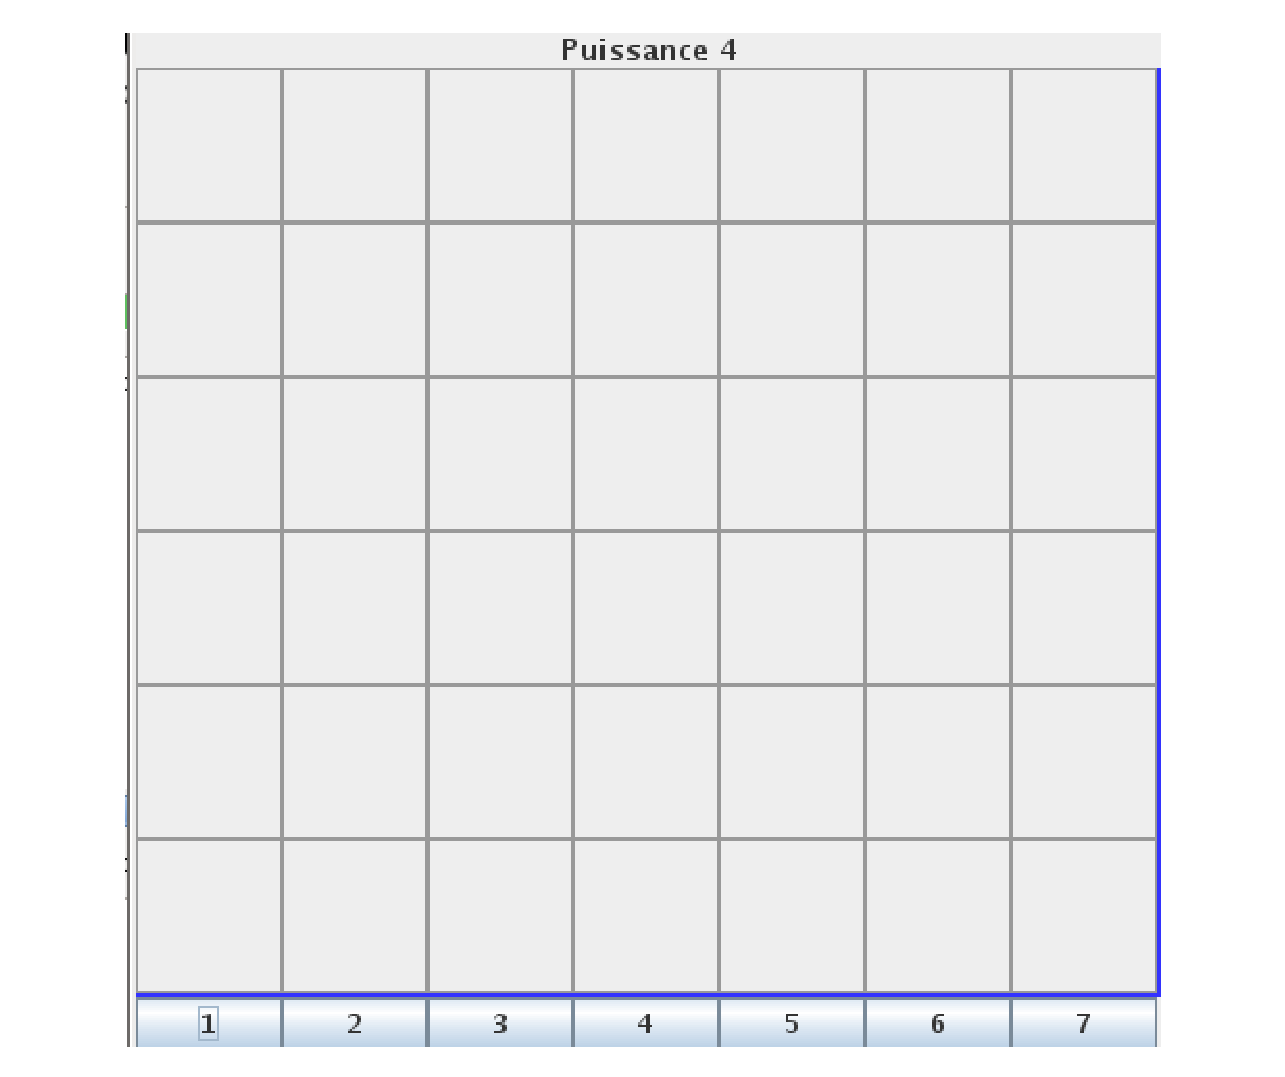
\includegraphics[scale=0.2]{nmfigempty}
  \caption{\texttt{Grille vide}}
\end{center}
\end{figure}

La grille est vide nous devons donc vérifier que l'ordinateur ne met pas encore en place de stratégie donc que 
\texttt{playable[]} est entièrement à 0 et que donc par défaut l'ordianteur joue au centre de la grille.


\begin{verbatim}
int Ia2Played = ia2.play(rule);
assertNotNull(Ia2Played);
assertTrue(0 <= Ia2Played && Ia2Played < grid.getWidth());
assertEquals(3, Ia2Played);
int[] playable2 = ia2.getPlayable();
for ( int i =0 ; i<ia2.getCpuGrid().getWidth();i++)
assertEquals(0,playable2[i]);
\end{verbatim}


\begin{figure}[H]
\begin{center}
  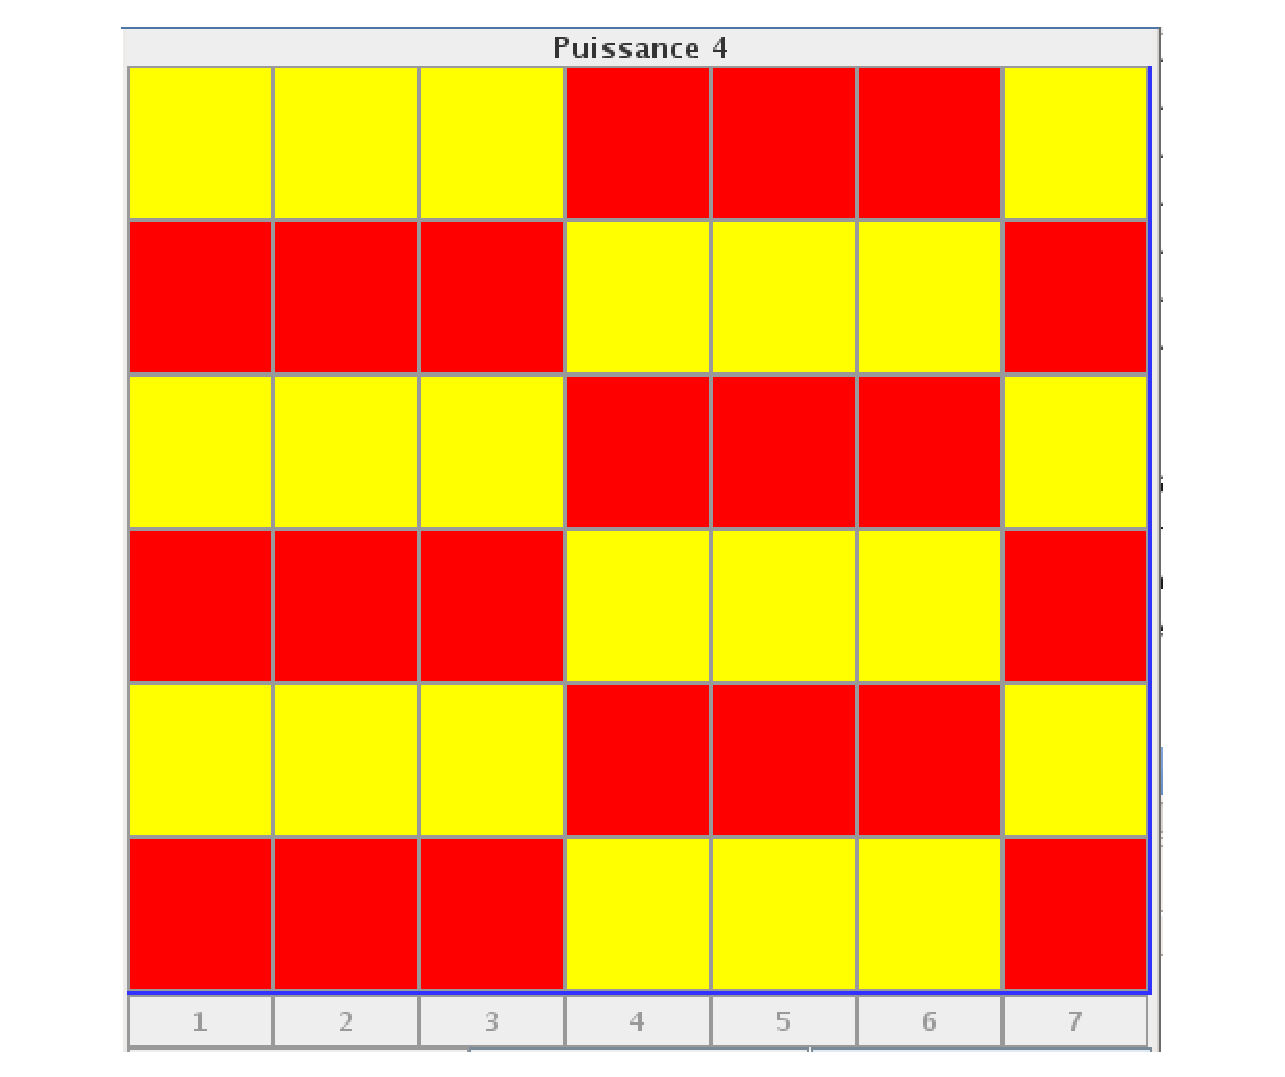
\includegraphics[scale=0.2]{nmfigfull}
  \caption{\texttt{Grille pleine}}
\end{center}
\end{figurre}

La grille étant pleine l'ordinateur ne peut donc pas jouer elle doit retrouner le code d'erreur -1.

\begin{verbatim}
 int Ia2PlayedFullGrid = ia2.play(rule);
 assertFalse(0 <= Ia2PlayedFullGrid && Ia2PlayedFullGrid < grid.getWidth());
 assertEquals(-1, Ia2PlayedFullGrid);
\end{verbatim}

\begin{figure}[H]
\begin{center}
  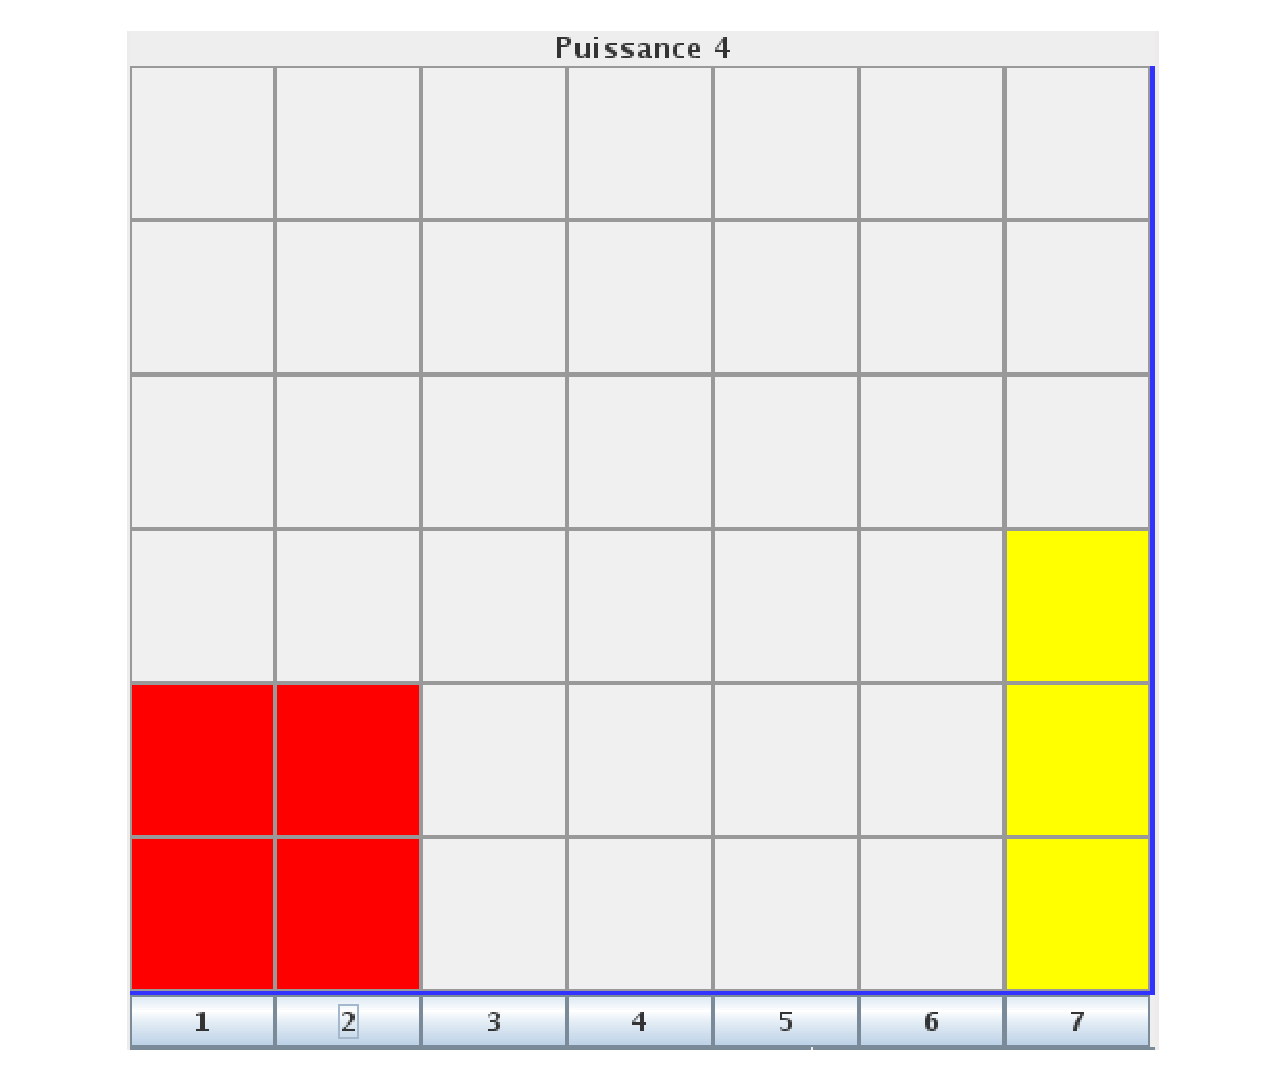
\includegraphics[scale=0.2]{nmfigwin}
  \caption{\texttt{Grille avec coup gagnant}}
\end{center}
\end{figurre}

Il y a la possibilité pour l'ordinateur de gagner elle doit donc repérer la collone qui permet de gagner en y mettant le code \texttt{playable} à 3 et y jouer.

\begin{verbatim}
 int Ia4PlayedForWin = ia4.play(rule);
assertNotNull(Ia4PlayedForWin);
assertTrue(0 <= Ia4PlayedForWin && Ia4PlayedForWin < grid_null.getWidth());
assertEquals(6, Ia4PlayedForWin);
int[] playable4 = ia4.getPlayable();
for ( int i =0 ; i<ia4.getCpuGrid().getWidth();i++)
   if ( i == 6)
assertEquals(3,playable4[i]);
   else
assertEquals(0,playable4[i]);
\end{verbatim}


\begin{figure}[H]
\begin{center}
  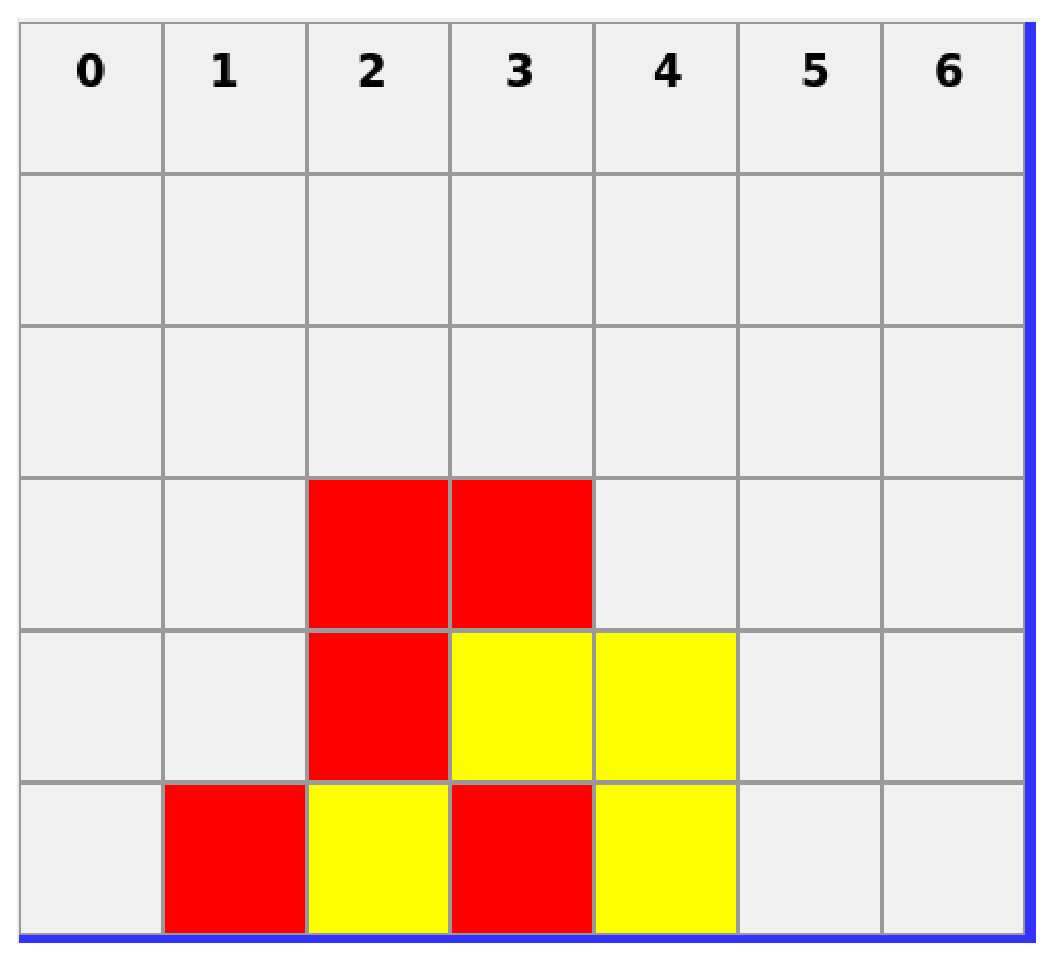
\includegraphics[scale=0.2]{playable10}
  \caption{\texttt{Colonne injouable}}
\end{center}
\end{figure}
Si l'ordinateur joue sur la colonne 4, alors au prochain coups le
joueur humain pourra gagner avec une diagonale. L'ordinateur devra donc avoir
\texttt{playable[4]=1} et jouer sur une autre case ici par la programmation nous savons qu'il va jouer en 2.

\begin{verbatim}
 int Ia2Playedfig2 = ia2.play(rule);
int[] playable5 = ia2.getPlayable();
assertEquals(2 , Ia2Playedfig2);
assertEquals(1 , playable5[4]);
\end{verbatim}


\begin{figure}[H]
\begin{center}
  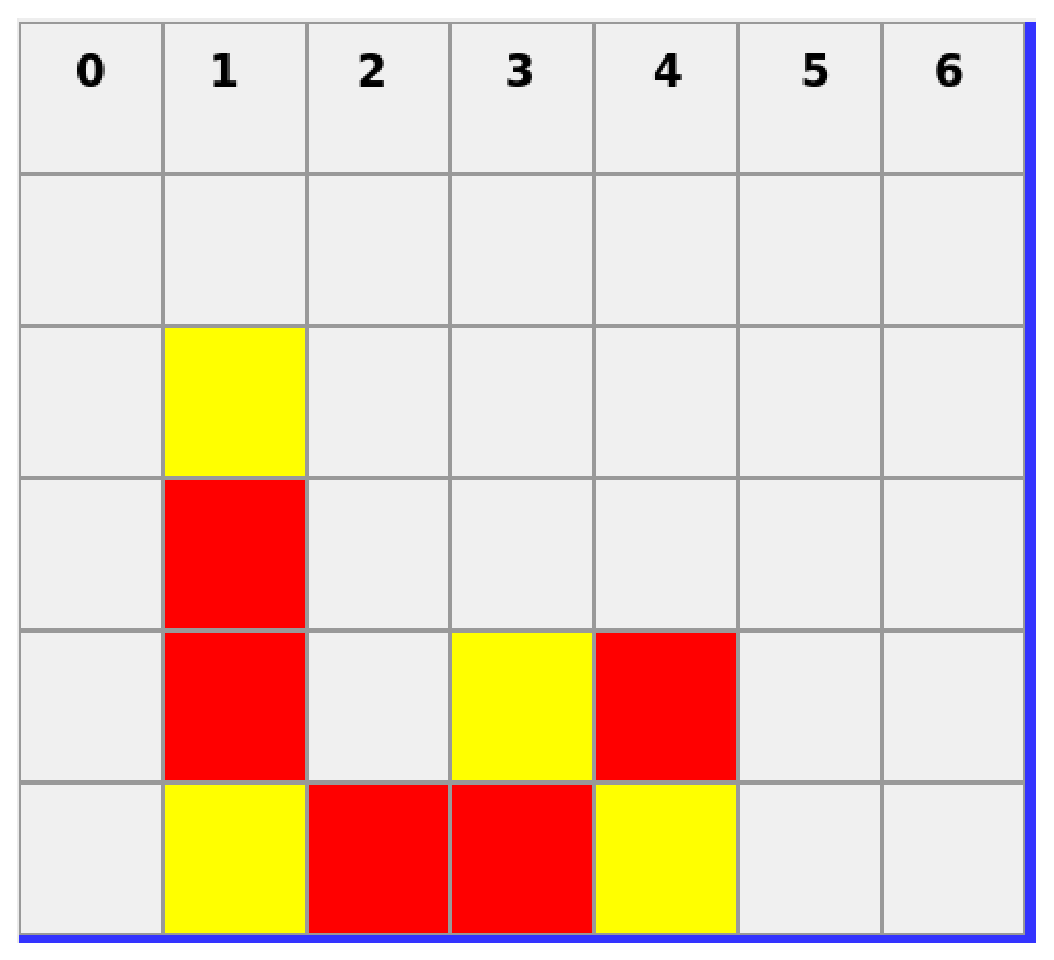
\includegraphics[scale=0.2]{playable2}
  \caption{\texttt{Strategie sur plusieur coups}}
\end{center}
\end{figure}
Si l'ordinateur joue en 2 cela permettra a l'humain de bloquer un coup gagnant 
l'ordinateur doit avoir \texttt{playable[2] = 2} ce qui est un code moins fort que 1 
mais il ne doit pas y jouer tout de même.

\begin{verbatim}
 int Ia2Playedfig3 = ia2.play(rule);
int[] playable6 = ia2.getPlayable();
assertEquals(3 , Ia2Playedfig3);
assertEquals(2, playable6[2]);
\end{verbatim}


\begin{figure}[H]
\begin{center}
  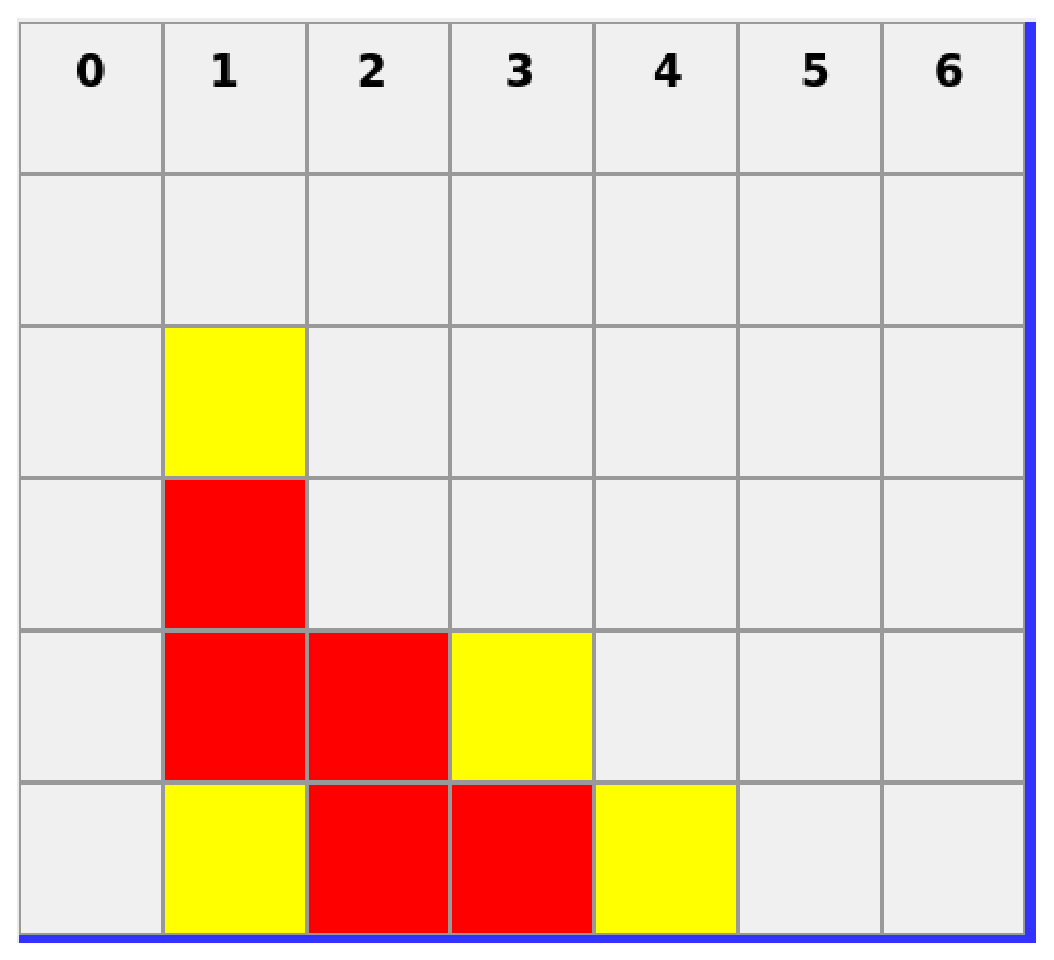
\includegraphics[scale=0.2]{playable3}
  \caption{\texttt{Autre cas de coup gagnant}}
\end{center}
\end{figure}
L'odinateur peut à nouveau gagner en jounant en jouant en 2.

\begin{verbatim}
 int Ia2Playedfig4 = ia2.play(rule);
int[] playable7 = ia2.getPlayable();
assertEquals(2 , Ia2Playedfig4);
assertEquals(3, playable7[2]);
\end{verbatim}


\begin{figure}[H]
\begin{center}
  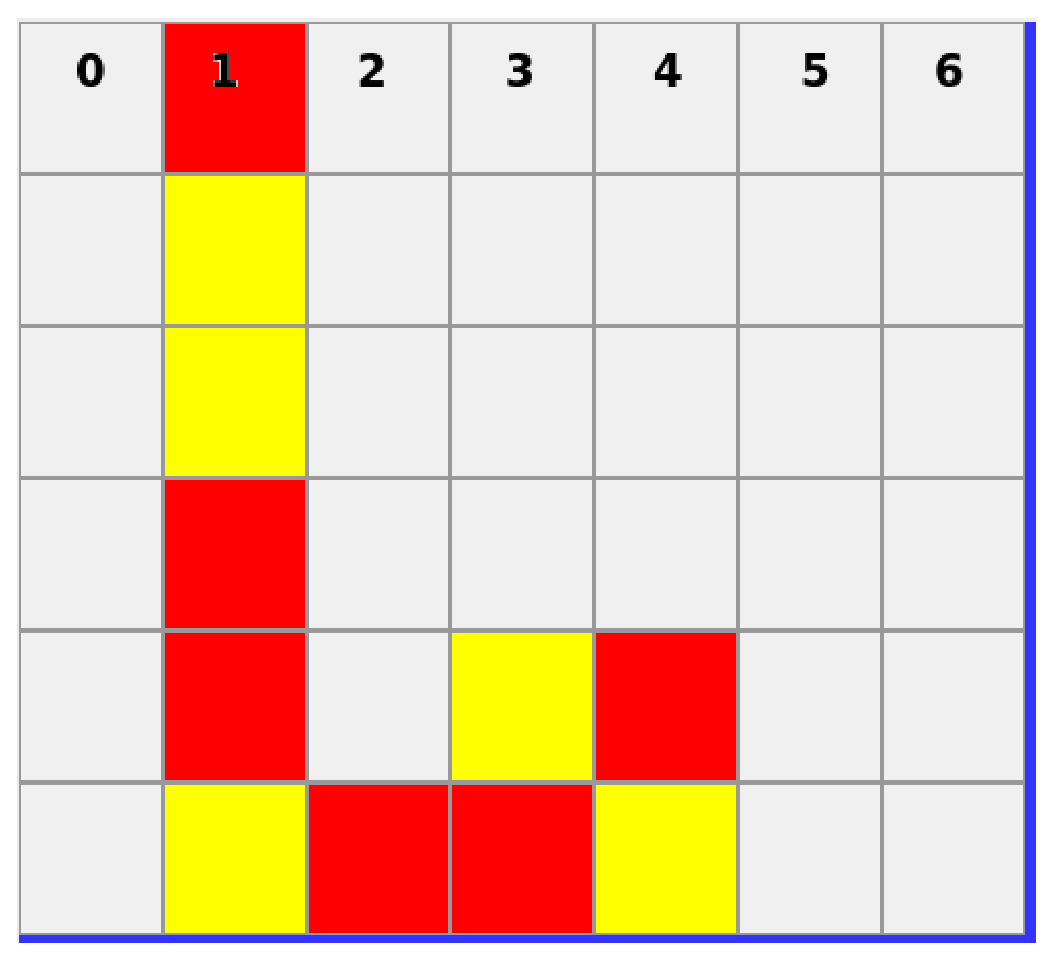
\includegraphics[scale=0.2]{playable4}
  \caption{\texttt{Colonne injouable}}
\end{center}
\end{figure}
La colonne 1 est pleine donc l'ordinateur ne doit plus y jouer et  \texttt{playable[1] = 4}.
C'est le code d'injouabilité le plus fort si tout les colonnes sont a 4 il renvera un code d'erreur -1.

\begin{verbatim}
 int[] playable8 = ia2.getPlayable();
assertEquals(4, playable8[1]);
\end{verbatim}


\begin{figure}[H]
\begin{center}
  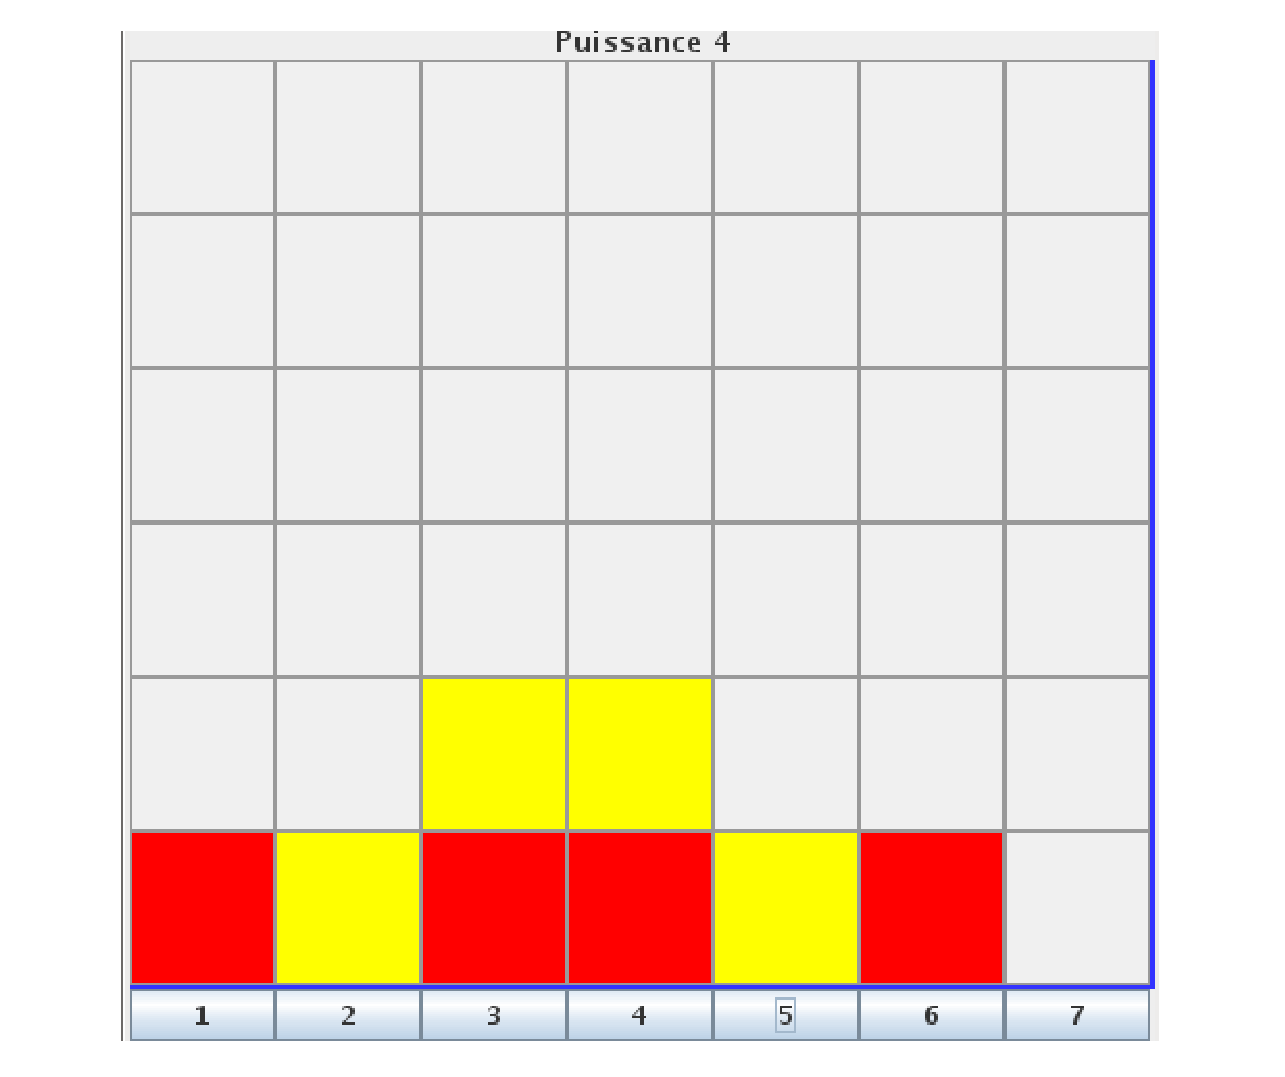
\includegraphics[scale=0.2]{nmfig6}
  \caption{\texttt{Strategie sur plusieurs coup}
\end{center}
\end{figure}
L'ordinateur doit remarquer qu'il peut gagner en deux coup il met donc \texttt{playable}
à 5 sur les cases offrant cette possibilitée : \texttt{playable[2] =  5} et \texttt{playable[5] = 5}.
(  colonne 2 et 6 sur la grille ).

\begin{verbatim}
 int Ia2Playedfig6 = ia2.play(rule);
int[] playable9 = ia2.getPlayable();
assertEquals(5 , Ia2Playedfig6);
assertEquals(5, playable9[1]);
assertEquals(5, playable9[5]);
\end{verbatim}


\begin{figure}[H]
\begin{center}
  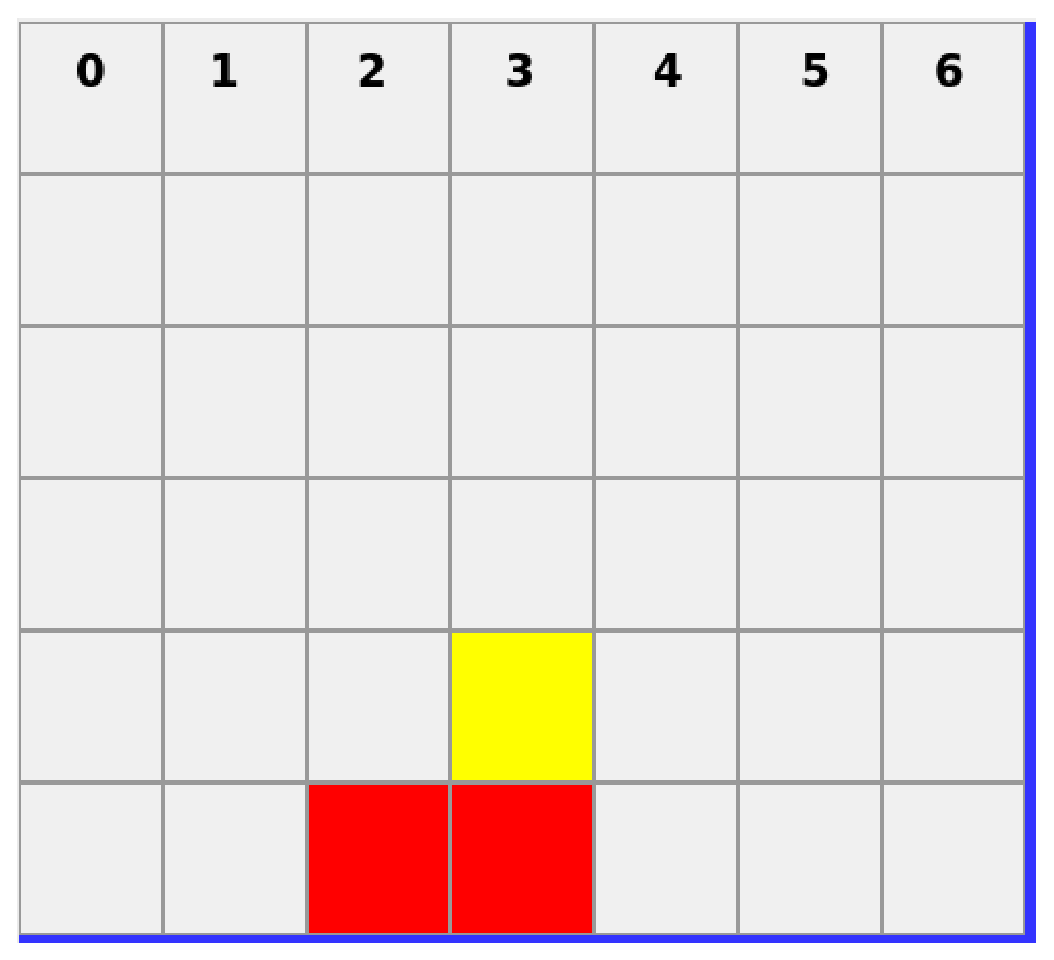
\includegraphics[scale=0.2]{playable1}
  \caption{\texttt{playable[i] = 6}}
\end{center}
\end{figure}
Dans ce cas la \texttt{playable[1] = 6} et \texttt{playable[4] = 6}. Et tous
les autres cas \texttt{playable[i]=0}. L'ordinateur va bloquer la
possibilit� de mouvement de l'humain.

\begin{figure}[H]
\begin{center}
  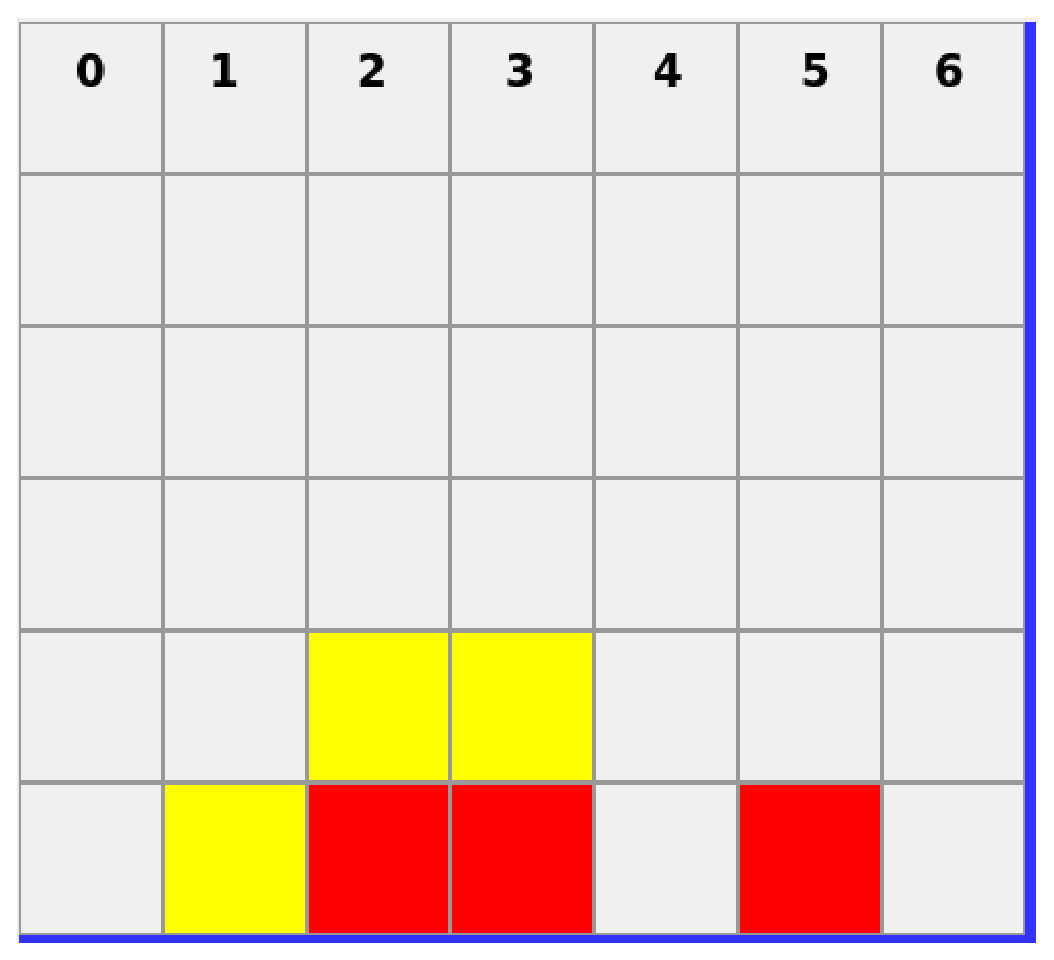
\includegraphics[scale=0.2]{playable6}
  \caption{\texttt{playable[i] = 6}}
\end{center}
\end{figure}
Si le joueur humain place un pion dans la colonne 4 il remportera la
victoire. Pour eviter de perdre aussi facilement on met
\texttt{playable[4]=6}, et l'ordinateur va bloquer la victoire du
joeur humain.


